\chapter{四足機械狗運動學模擬}

通過運動學模擬可以找出最大受力點及作動角度範圍、姿態使其符合設計需求。

%-------------硬體架構-----------------%
\section{硬體架構}

馬達(一):\
所帶動的A桿件,此A為兩個部分組成,其一為固定馬達的零件A-1與之結合的為A-2,兩個零件結合能夠為桿件D提供支撐及限制運動狀態,使D桿件只能做搖擺運動,得益於A的粗壯,讓整體連桿能提供良好的穩定性及負載。\\
馬達(二):\
所帶動的D桿件,因為A得角度和旋轉限制,使其只能做搖擺運動,D桿件在搖擺後將帶動C桿件,此力在傳遞到B桿件(小腿),使其也能做搖擺運動。\
由於A桿件跟著搖擺,大大的增加了此步行機構的運動姿態,B桿末端點有著更大的自由度,可以對應不同地形及運動狀態,但是此機構因此對設計及控制精度的要求更高。\\

\begin{figure}[hbt!]
\begin{center}
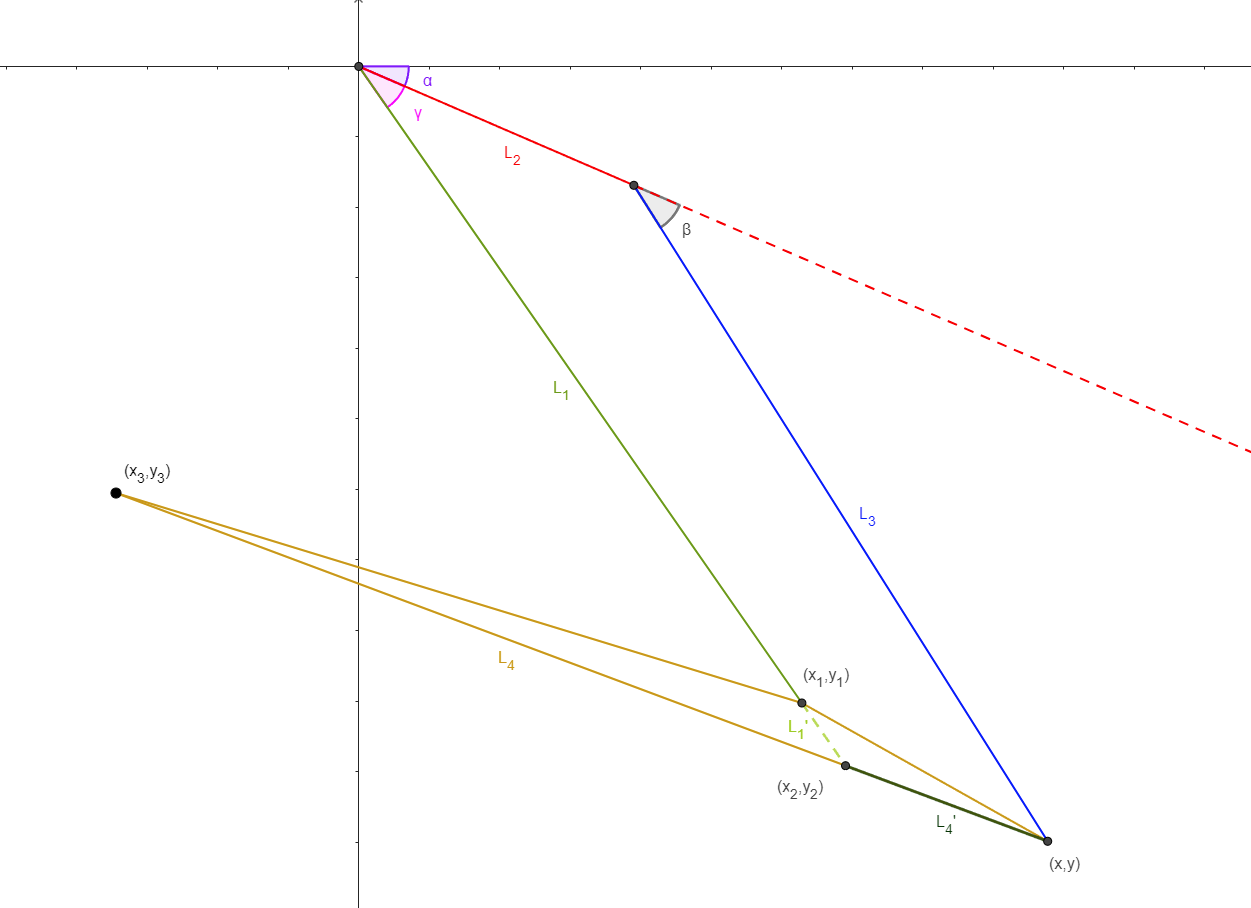
\includegraphics[angle=90,width=10cm]{Forward kinematics formula}
\caption{\Large 四連趕機構}\label{Forward kinematics formula}
\end{center}
\end{figure}

A部分:Leg1-1 + Leg1-5
B部分:Leg2 + Leg3
C部分:leg4

 %------------軟體架構-----------------%
\section{Python控制程式}
運動模擬主要以Python程式碼進行控制,而程式碼部分我們選擇利用鍵盤控制模型的動作,首先導入模塊(API模塊: 遠端通訊、keyboard模塊: 檢測鍵盤輸入、time模塊: 暫停當前程式一段時間)。\\
導入控制的主機位置,創建一個從遠端客戶端獲取的對象的變量,進行運動模擬控制,在軟體控制中,我們利用角度控制轉軸的所在位置,首先調用需要控制的轉軸,接著定義控制轉軸的函數,設置無限迴圈檢測目標按鍵為正確位置,再將先前定義的函數寫入迴圈,以上步驟完成後,即可控制每隻轉軸角度達成理想動作。\\
設定前進動作時,先將左前腿及右後腿往前抬,並同時將右前腿及左後腿往後踢設定前抬左前腿時,左前腿的前抬角度必須比右後腿高,這樣才不會使左前腿觸碰到地面而造成反力無法前進。\\
設定後退動作:先將左前腿及右後腿往後抬,同時將右前腿及左後腿往前踢,設定後抬右後腿時,右後腿的後抬角度必須比左前腿高,這樣才不會使右後腿觸碰到地面而造成反力無法後退,完成前面的動作後,將左右動作對調即可達成左右腿互換的動作。\\

\newpage

%-----------運動學模擬------------%
\section{運動模擬}
首先將模型轉化成STL檔案使其能被CoppeliaSim開啟,利用移動功能將模型移動至合適位置,點選模型使用爆炸功能將模型由一體分為數個零件,插入轉軸並設定中修改零件的重量等參數,導入Pythan程式碼,使用播放查看個機件的姿態、作動是否符合設計,完成之後就可以對模型進行分析並帶入負載求解。\\

動態模擬結束後,我們可以將四足機器人運動模式分為以下三種,分別為:\
\begin{enumerate}
\item 爬行(Crawl):\
此動作較簡單且容易控制,作用在於機器人需緩慢移動或是穩定度需求高的情況下,由其中單腳前伸其餘進行關節旋轉,在小位移量的情況下實現行走功能。\\
\item 小跑(Trot):\
此作用型態為FR+RL或FL+RR做動,進行移動時有著兩動兩不動的準則,在不動的部分做關節的旋轉運動,令四足機器人在快速移動下還能對身體保持平衡,在大位移量的情況下實現行走功能。\\
\item 跳躍(Bound):\
由前兩足進行快速彈跳位移,使機器狗的關節進行快速調整以支撐身體姿態,分為FL+FR及RL+RR兩組,在躍障或其他特殊行為中使用。\\
\end{enumerate}
\begin{figure}[htbp]
  \centering
  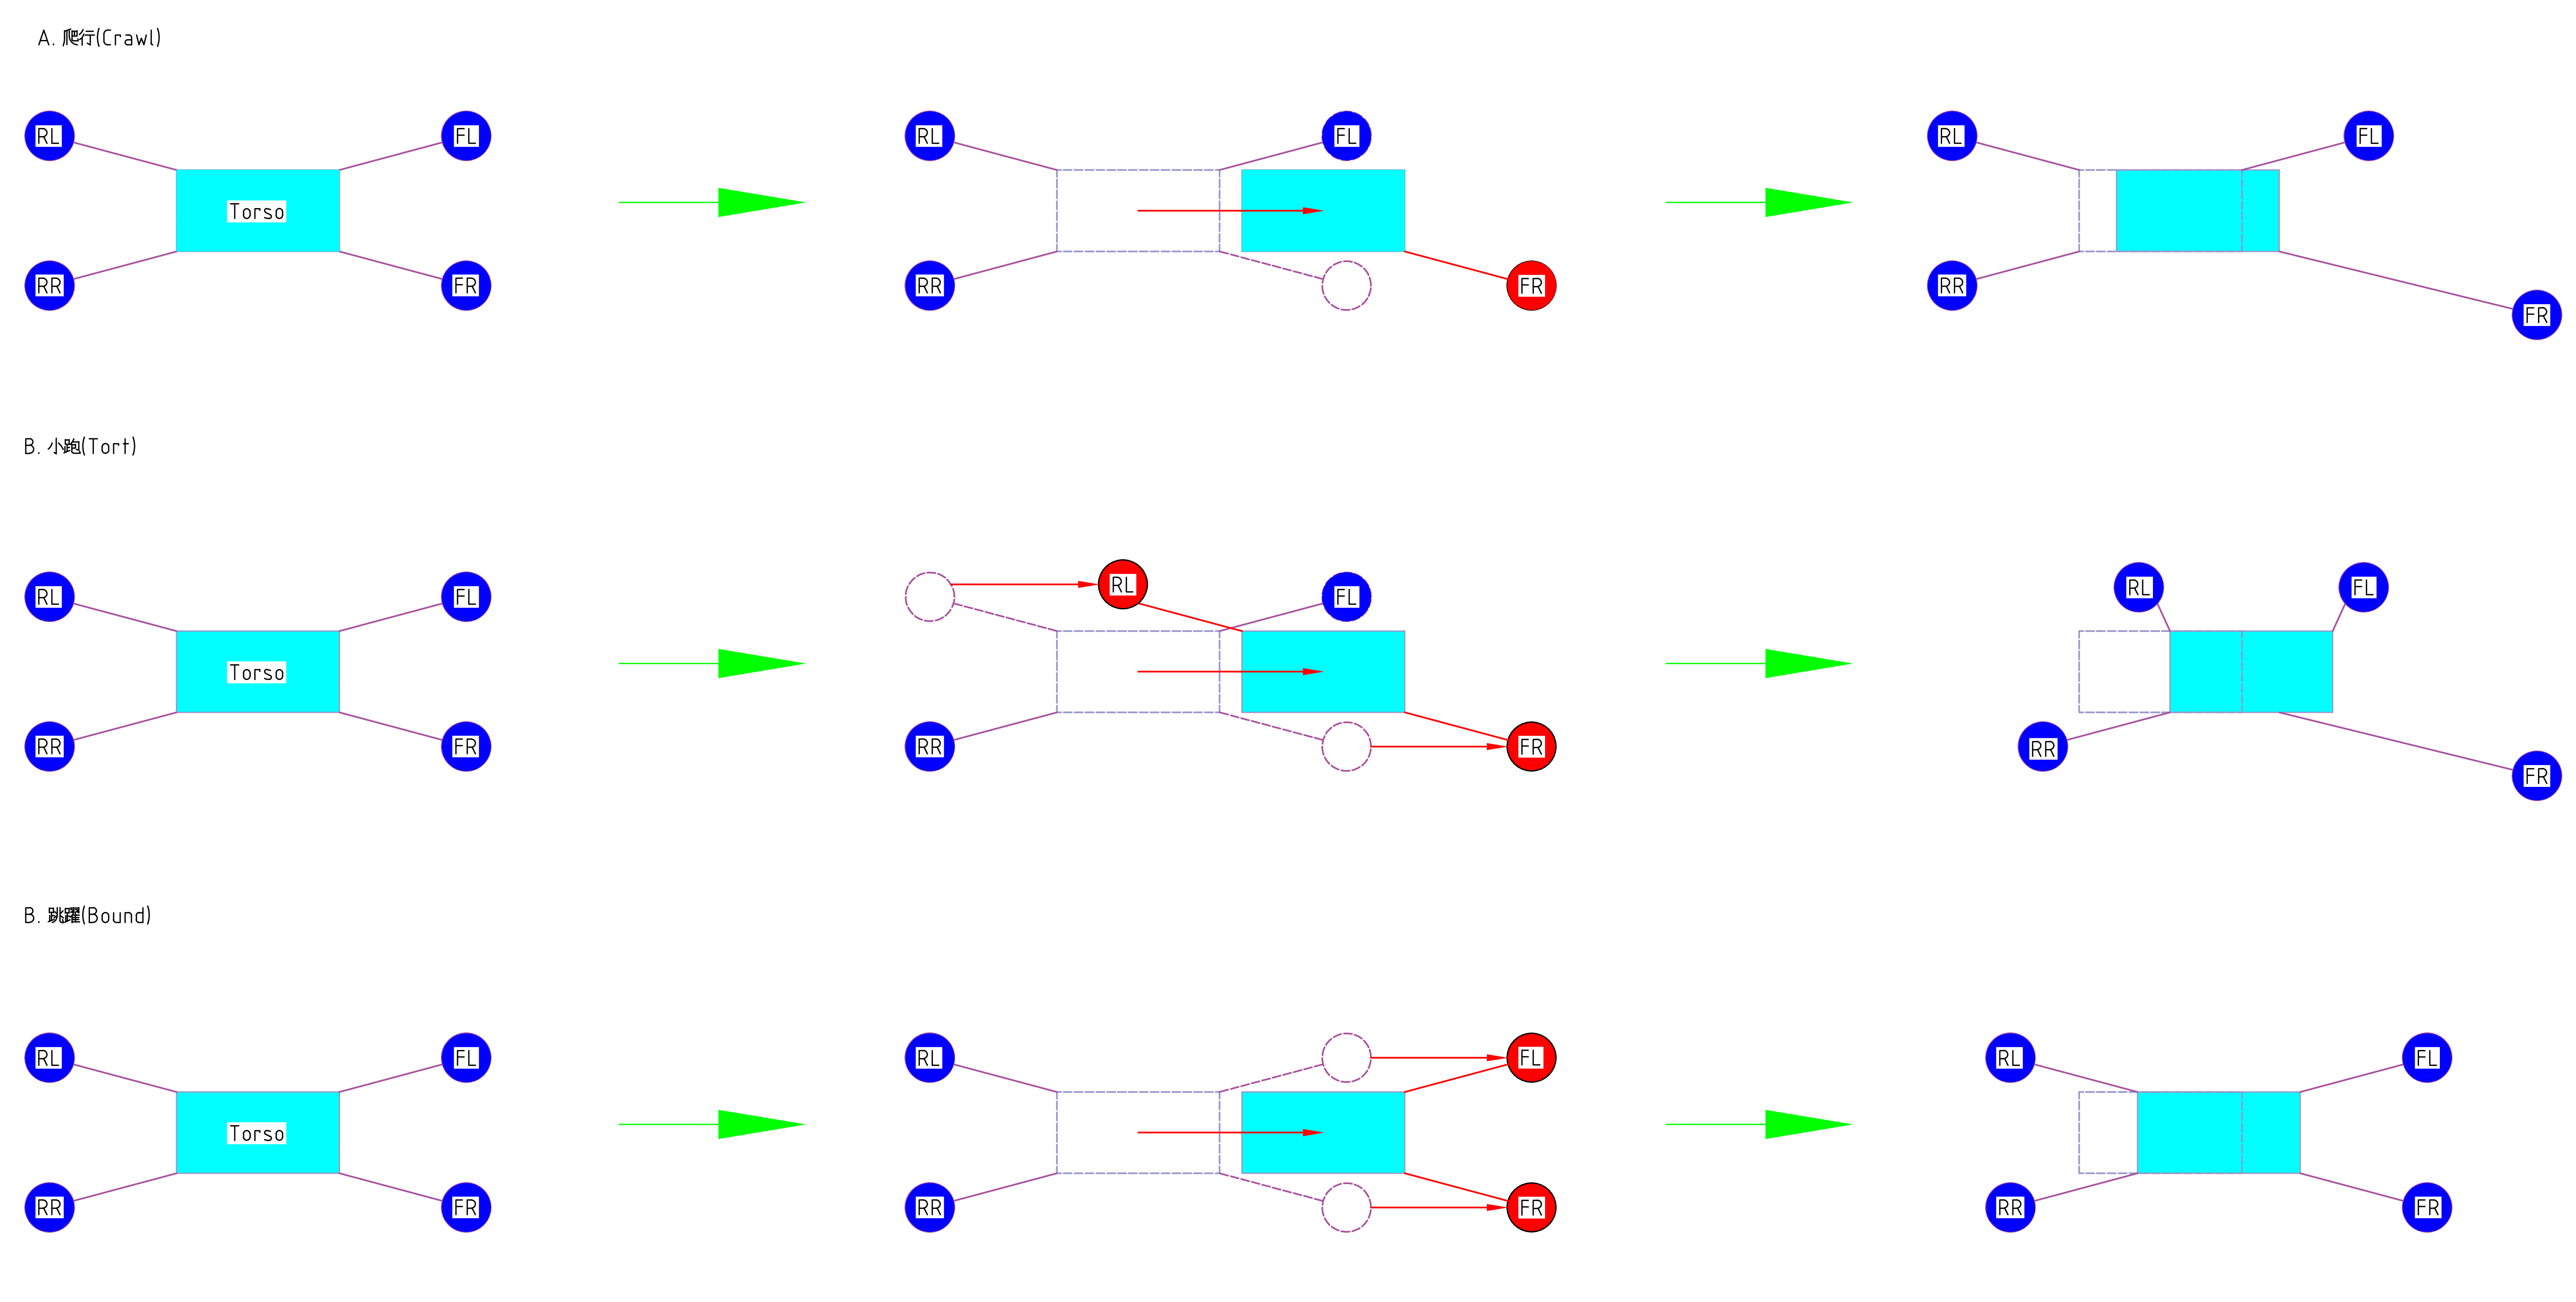
\includegraphics[width=\textwidth]{各式步態圖}
  \caption{各式步態圖}
  \label{各式步態圖}
\end{figure}
\newpage
